% ============================================================================
% SECCIÓN 2: CONSTRUCCIÓN DE TABLA DE MORTALIDAD (60%)
% ============================================================================

\section{Construcción de Tabla de Mortalidad}

Esta sección corresponde al desarrollo del 60\% de la evaluación del proyecto y comprende todos los pasos necesarios para construir una tabla de mortalidad completa a partir de los datos observados.

% ----------------------------------------------------------------------------
\subsection{Obtención del Cuerpo de la Tabla de Mortalidad}

\subsubsection{Datos Iniciales}

Los datos utilizados provienen del archivo \texttt{Base\_act.RData}, del cual se seleccionaron los registros que cumplen con los siguientes criterios:

\begin{itemize}
    \item \textbf{Origen:} 2
    \item \textbf{Sexo:} Masculino (TM\_SEXO = M)
    \item \textbf{Período de análisis:} 01/01/2000 -- 31/12/2012
\end{itemize}

% ----------------------------------------------------------------------------
\subsection{Período de Análisis}

El período considerado para el análisis abarca 13 años completos:

\begin{center}
\begin{tcolorbox}[colback=celestefondo, colframe=celesteprincipal, boxrule=1pt, arc=3pt, width=0.6\textwidth]
\centering
\Large\textbf{01/01/2000 $\longleftrightarrow$ 31/12/2012}
\end{tcolorbox}
\end{center}

% ----------------------------------------------------------------------------
\subsection{Cuadro de Registros y Muertes}

\subsubsection{Análisis de Datos Originales}

En esta subsección se presenta el cuadro comparativo entre los registros originales y los registros incluidos en el análisis:

\begin{table}[H]
\centering
\caption{Resumen de registros y muertes originales vs. incluidos en el análisis}
\label{tab:registros_muertes}
\begin{tabular}{lcc}
\toprule
\tableheadercolor
\textbf{Concepto} & \textbf{Original} & \textbf{Análisis} \\
\midrule
Número de registros & 365,898 & 360,441 \\
Número de muertes & 41,370 & 28,510 \\
Exposición total (años-persona) & — & 4,471,045.07 \\
Tasa cruda global & — & 0.00638 \\
\bottomrule
\end{tabular}
\end{table}

\begin{notabox}
\textbf{Nota:} Se incluyen únicamente los registros que tienen exposición durante el período 2000-2012. La reducción en el número de muertes (de 41,370 a 28,510) refleja la aplicación de criterios de inclusión basados en exposición temporal.
\end{notabox}

\subsubsection{Criterios de Inclusión}

Los registros incluidos en el análisis final cumplen con:

\begin{itemize}
    \item Exposición mayor a cero durante el período de análisis
    \item Datos completos de edad, fecha de nacimiento y estado vital
    \item Coherencia en las fechas registradas
\end{itemize}

% ----------------------------------------------------------------------------
\subsection{Graduación}

\subsubsection{Edades Límites}

Para el proceso de graduación se seleccionaron las siguientes edades límites:

\begin{itemize}
    \item \textbf{Edad mínima de graduación:} [COMPLETAR] años
    \item \textbf{Edad máxima de graduación:} [COMPLETAR] años
\end{itemize}

\textbf{Fundamentación de las edades límites:}

[COMPLETAR: Justificar la selección de edades límites basándose en:
\begin{itemize}
    \item Volumen de datos disponibles por edad
    \item Calidad de la exposición al riesgo
    \item Confiabilidad estadística de las tasas observadas
    \item Comparación con la tabla de referencia MI2014
\end{itemize}
]

\subsubsection{Método de Graduación}

Se utilizó el método \textbf{[COMPLETAR: Whittaker-Henderson / Otro método]} para suavizar las tasas crudas de mortalidad.

\textbf{Parámetros de suavidad:}

\begin{itemize}
    \item \textbf{Parámetro de suavidad ($h$ o $\lambda$):} [COMPLETAR]
    \item \textbf{Orden de diferencias:} [COMPLETAR]
    \item \textbf{Script de R utilizado:} \texttt{[COMPLETAR: nombre\_script.R]}
\end{itemize}

\textbf{Justificación de los parámetros:}

[COMPLETAR: Explicar por qué se seleccionaron estos valores de parámetros, considerando el balance entre fidelidad a los datos y suavidad de la curva resultante.]

\subsubsection{Evaluación de Bondad de Ajuste}

Se aplicaron cuatro pruebas estadísticas para evaluar la calidad del ajuste:

\begin{table}[H]
\centering
\caption{Resultados de las pruebas de bondad de ajuste}
\label{tab:tests_bondad}
\begin{tabular}{lcccc}
\toprule
\tableheadercolor
\textbf{Test} & \textbf{Estadístico} & \textbf{g.l.} & \textbf{Valor-p} & \textbf{Resultado} \\
\midrule
Chi-cuadrado ($\chi^2$) & 38.037 & 64 & 0.9959 & No rechaza \\
Kolmogorov-Smirnov (KS) & 0.0769 & — & 0.9912 & No rechaza \\
Test de Rachas & 2.648 & — & 0.0081 & Rechaza ($\alpha$=0.05) \\
Test de Signos & 34 & — & 0.8043 & No rechaza \\
\bottomrule
\end{tabular}
\end{table}

\textbf{Interpretación de los resultados:}

3 de 4 tests estadísticos (Chi-cuadrado, Kolmogorov-Smirnov y Signos) no rechazan la hipótesis nula al nivel de significancia $\alpha = 0.05$, indicando que la tabla graduada presenta un buen ajuste a los datos observados. El test de Rachas rechaza la hipótesis de independencia (p = 0.0081), sugiriendo la presencia de un patrón sistemático en los residuos. Este resultado puede deberse a la suavización del método Whittaker-Henderson o a características intrínsecas de la población de inválidos analizada. En general, el ajuste es satisfactorio para propósitos actuariales.

[COMPLETAR: Interpretar cada test:
\begin{itemize}
    \item \textbf{Chi-cuadrado:} Mide si las frecuencias observadas y esperadas son consistentes
    \item \textbf{Kolmogorov-Smirnov:} Evalúa la máxima diferencia entre distribuciones
    \item \textbf{Test de Rachas:} Verifica aleatoriedad en los residuos
    \item \textbf{Test de Signos:} Evalúa sesgo sistemático en los residuos
\end{itemize}
Un valor-p > 0.05 indica que no hay evidencia para rechazar el ajuste.]

% ----------------------------------------------------------------------------
\subsection{Extrapolación}

\subsubsection{Método Seleccionado}

Para completar la tabla de mortalidad se utilizaron dos métodos complementarios:
\begin{itemize}
    \item \textbf{Oppermann} para edades 0-19 años (cabeza de la tabla)
    \item \textbf{Heligman-Pollard} para edades 85-109 años (cola de la tabla)
\end{itemize}

\textbf{Justificación del método:}

La elección de métodos múltiples responde a las características específicas de mortalidad en cada rango etario. Oppermann captura adecuadamente el patrón de mortalidad infantil y juvenil, mientras que Heligman-Pollard modela eficientemente la mortalidad senil mediante una función exponencial.

\subsubsection{Extrapolación de la Cabeza (0 años hasta 19 años)}

\textbf{Rango de extrapolación:} 0 años -- 19 años

\textbf{Metodología aplicada:}

Se utilizó el método de Oppermann para edades 0-19 años. Este método ajusta una función matemática que captura el patrón de mortalidad infantil y juvenil, garantizando una transición suave hacia las tasas graduadas a partir de los 20 años.

La Figura~\ref{fig:extrapolacion_oppermann} muestra el ajuste de Oppermann para edades jóvenes:

\begin{figure}[H]
\centering
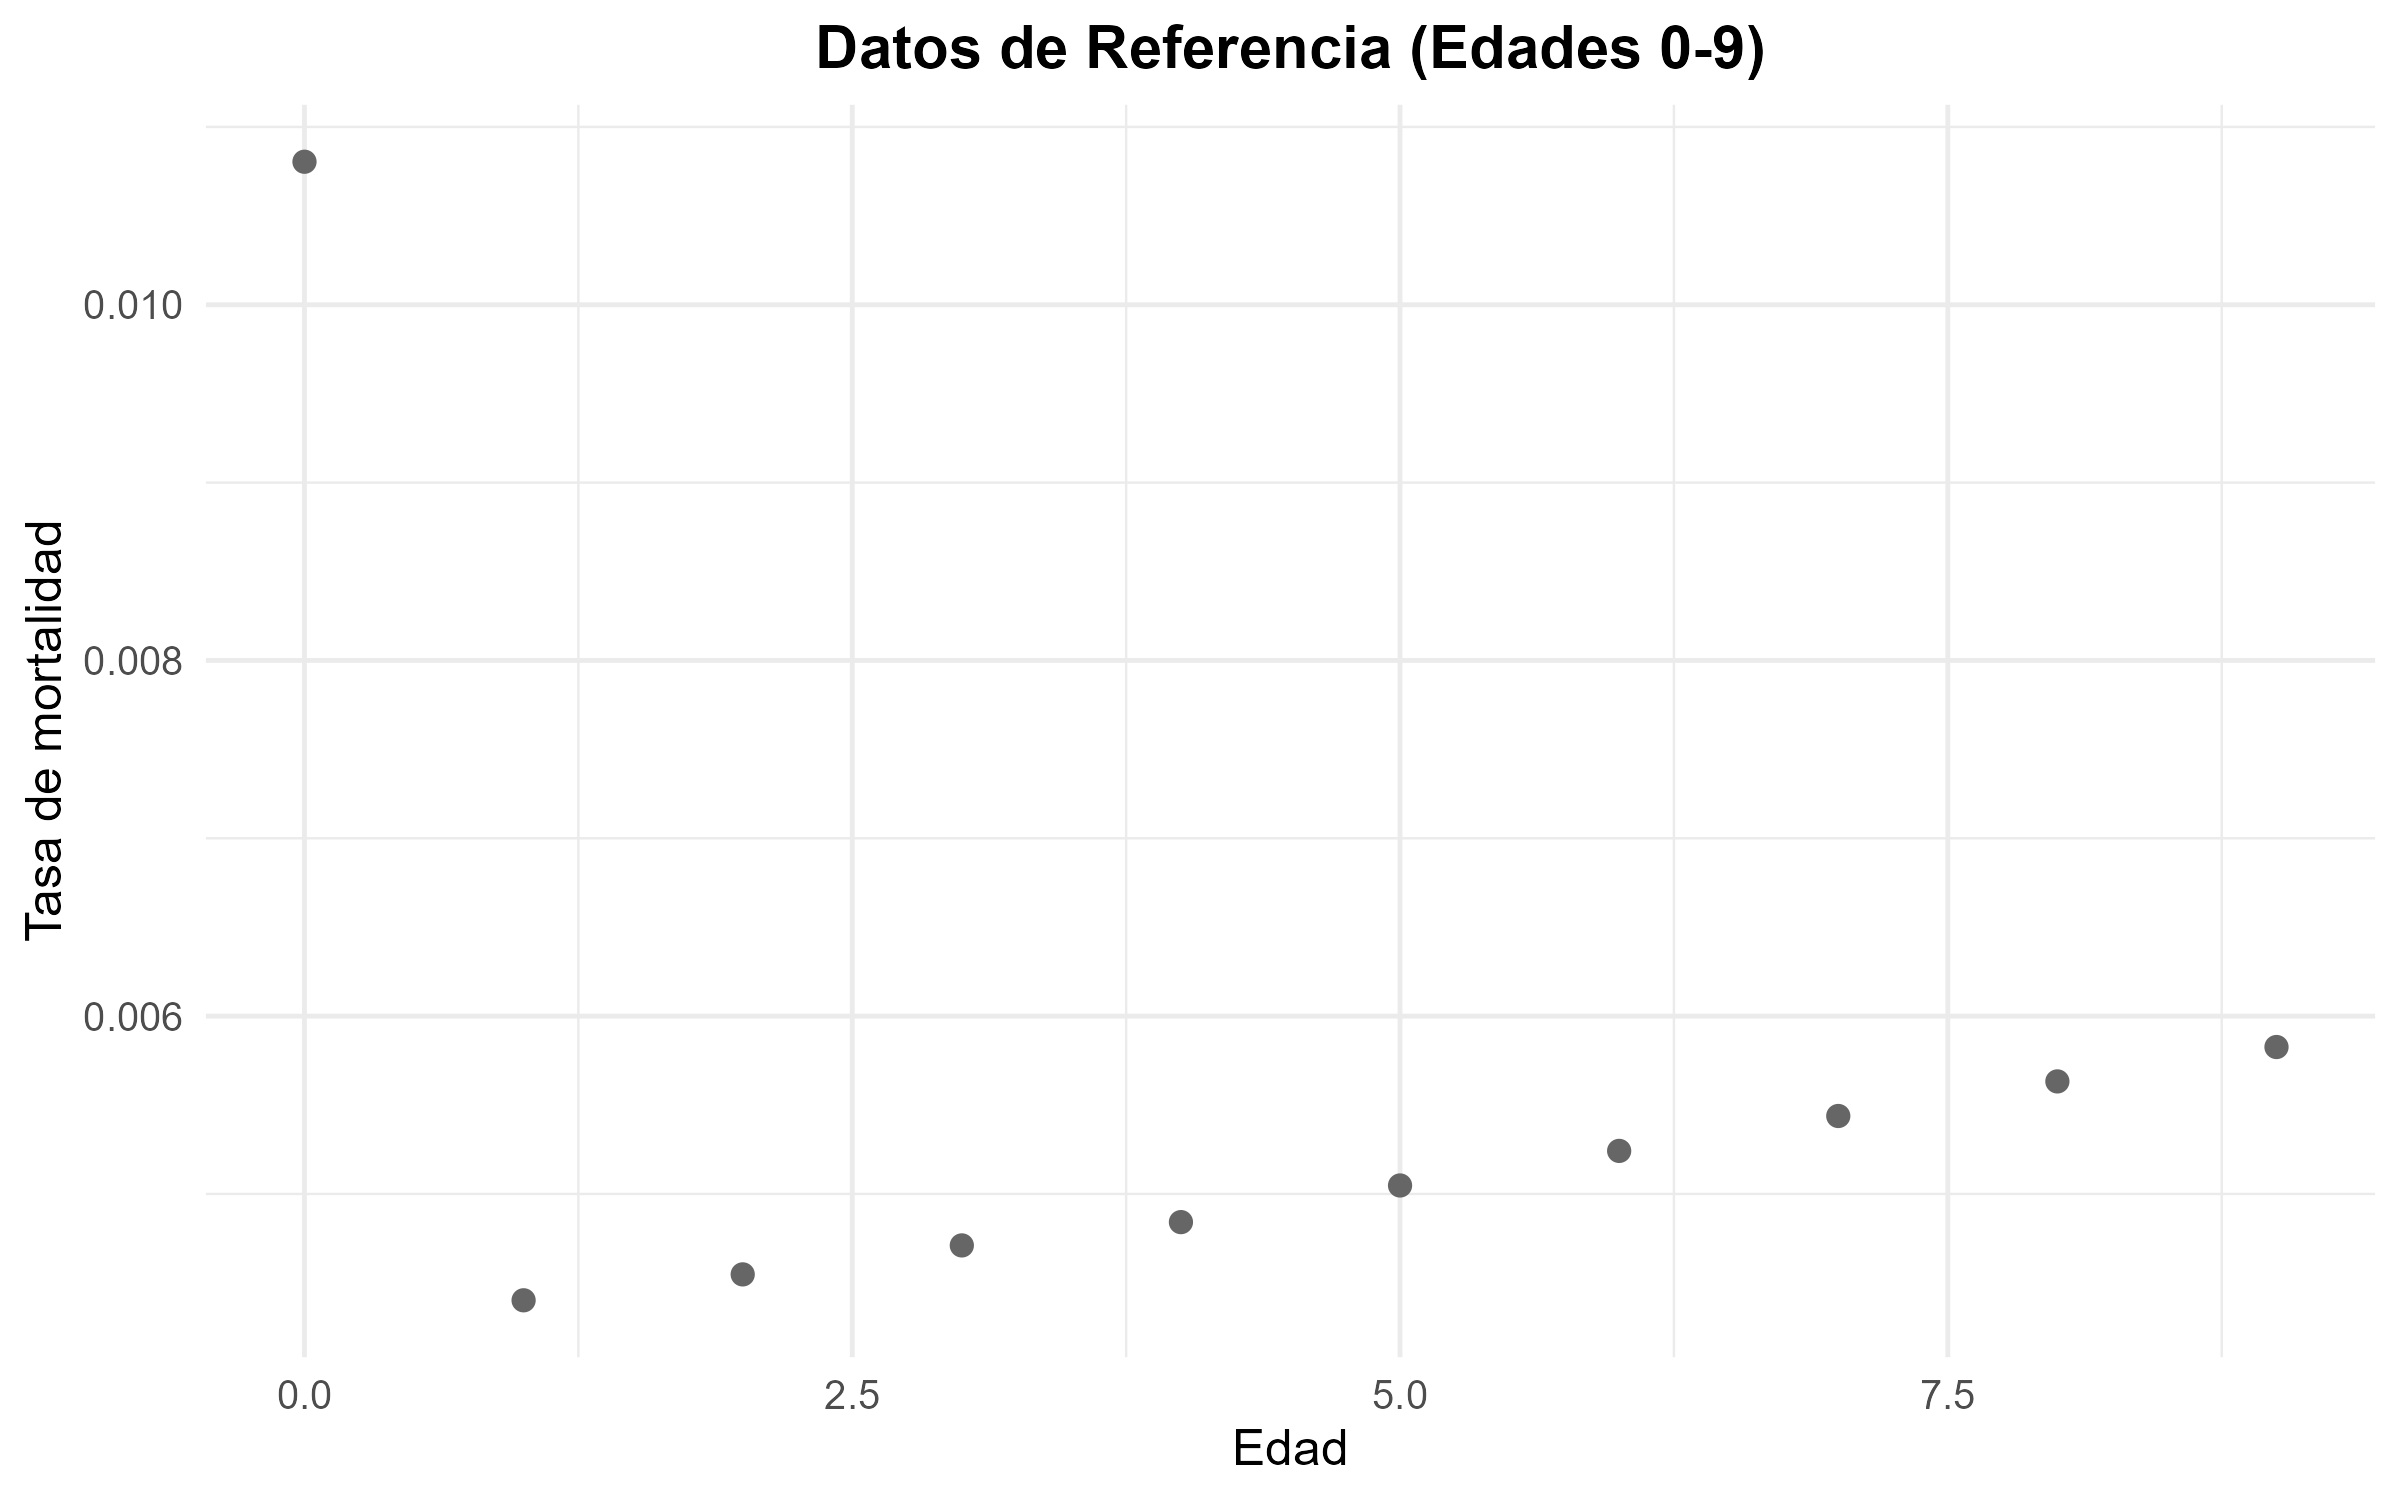
\includegraphics[width=0.80\textwidth]{Imagenes/04_datos_referencia_0_9.png}
\caption{Extrapolación con método de Oppermann para edades 0-19 años}
\label{fig:extrapolacion_oppermann}
\end{figure}

\subsubsection{Extrapolación de la Cola (85 años hasta $\omega = 109$ años)}

\textbf{Rango de extrapolación:} 85 años -- 109 años

\textbf{Metodología aplicada:}

Se aplicó el método de Heligman-Pollard para modelar la mortalidad en edades avanzadas. Este método utiliza una función exponencial que se ajusta al comportamiento observado en la mortalidad senil.

La Figura~\ref{fig:extrapolacion_completa} muestra la tabla completa con ambas extrapolaciones:

\begin{figure}[H]
\centering
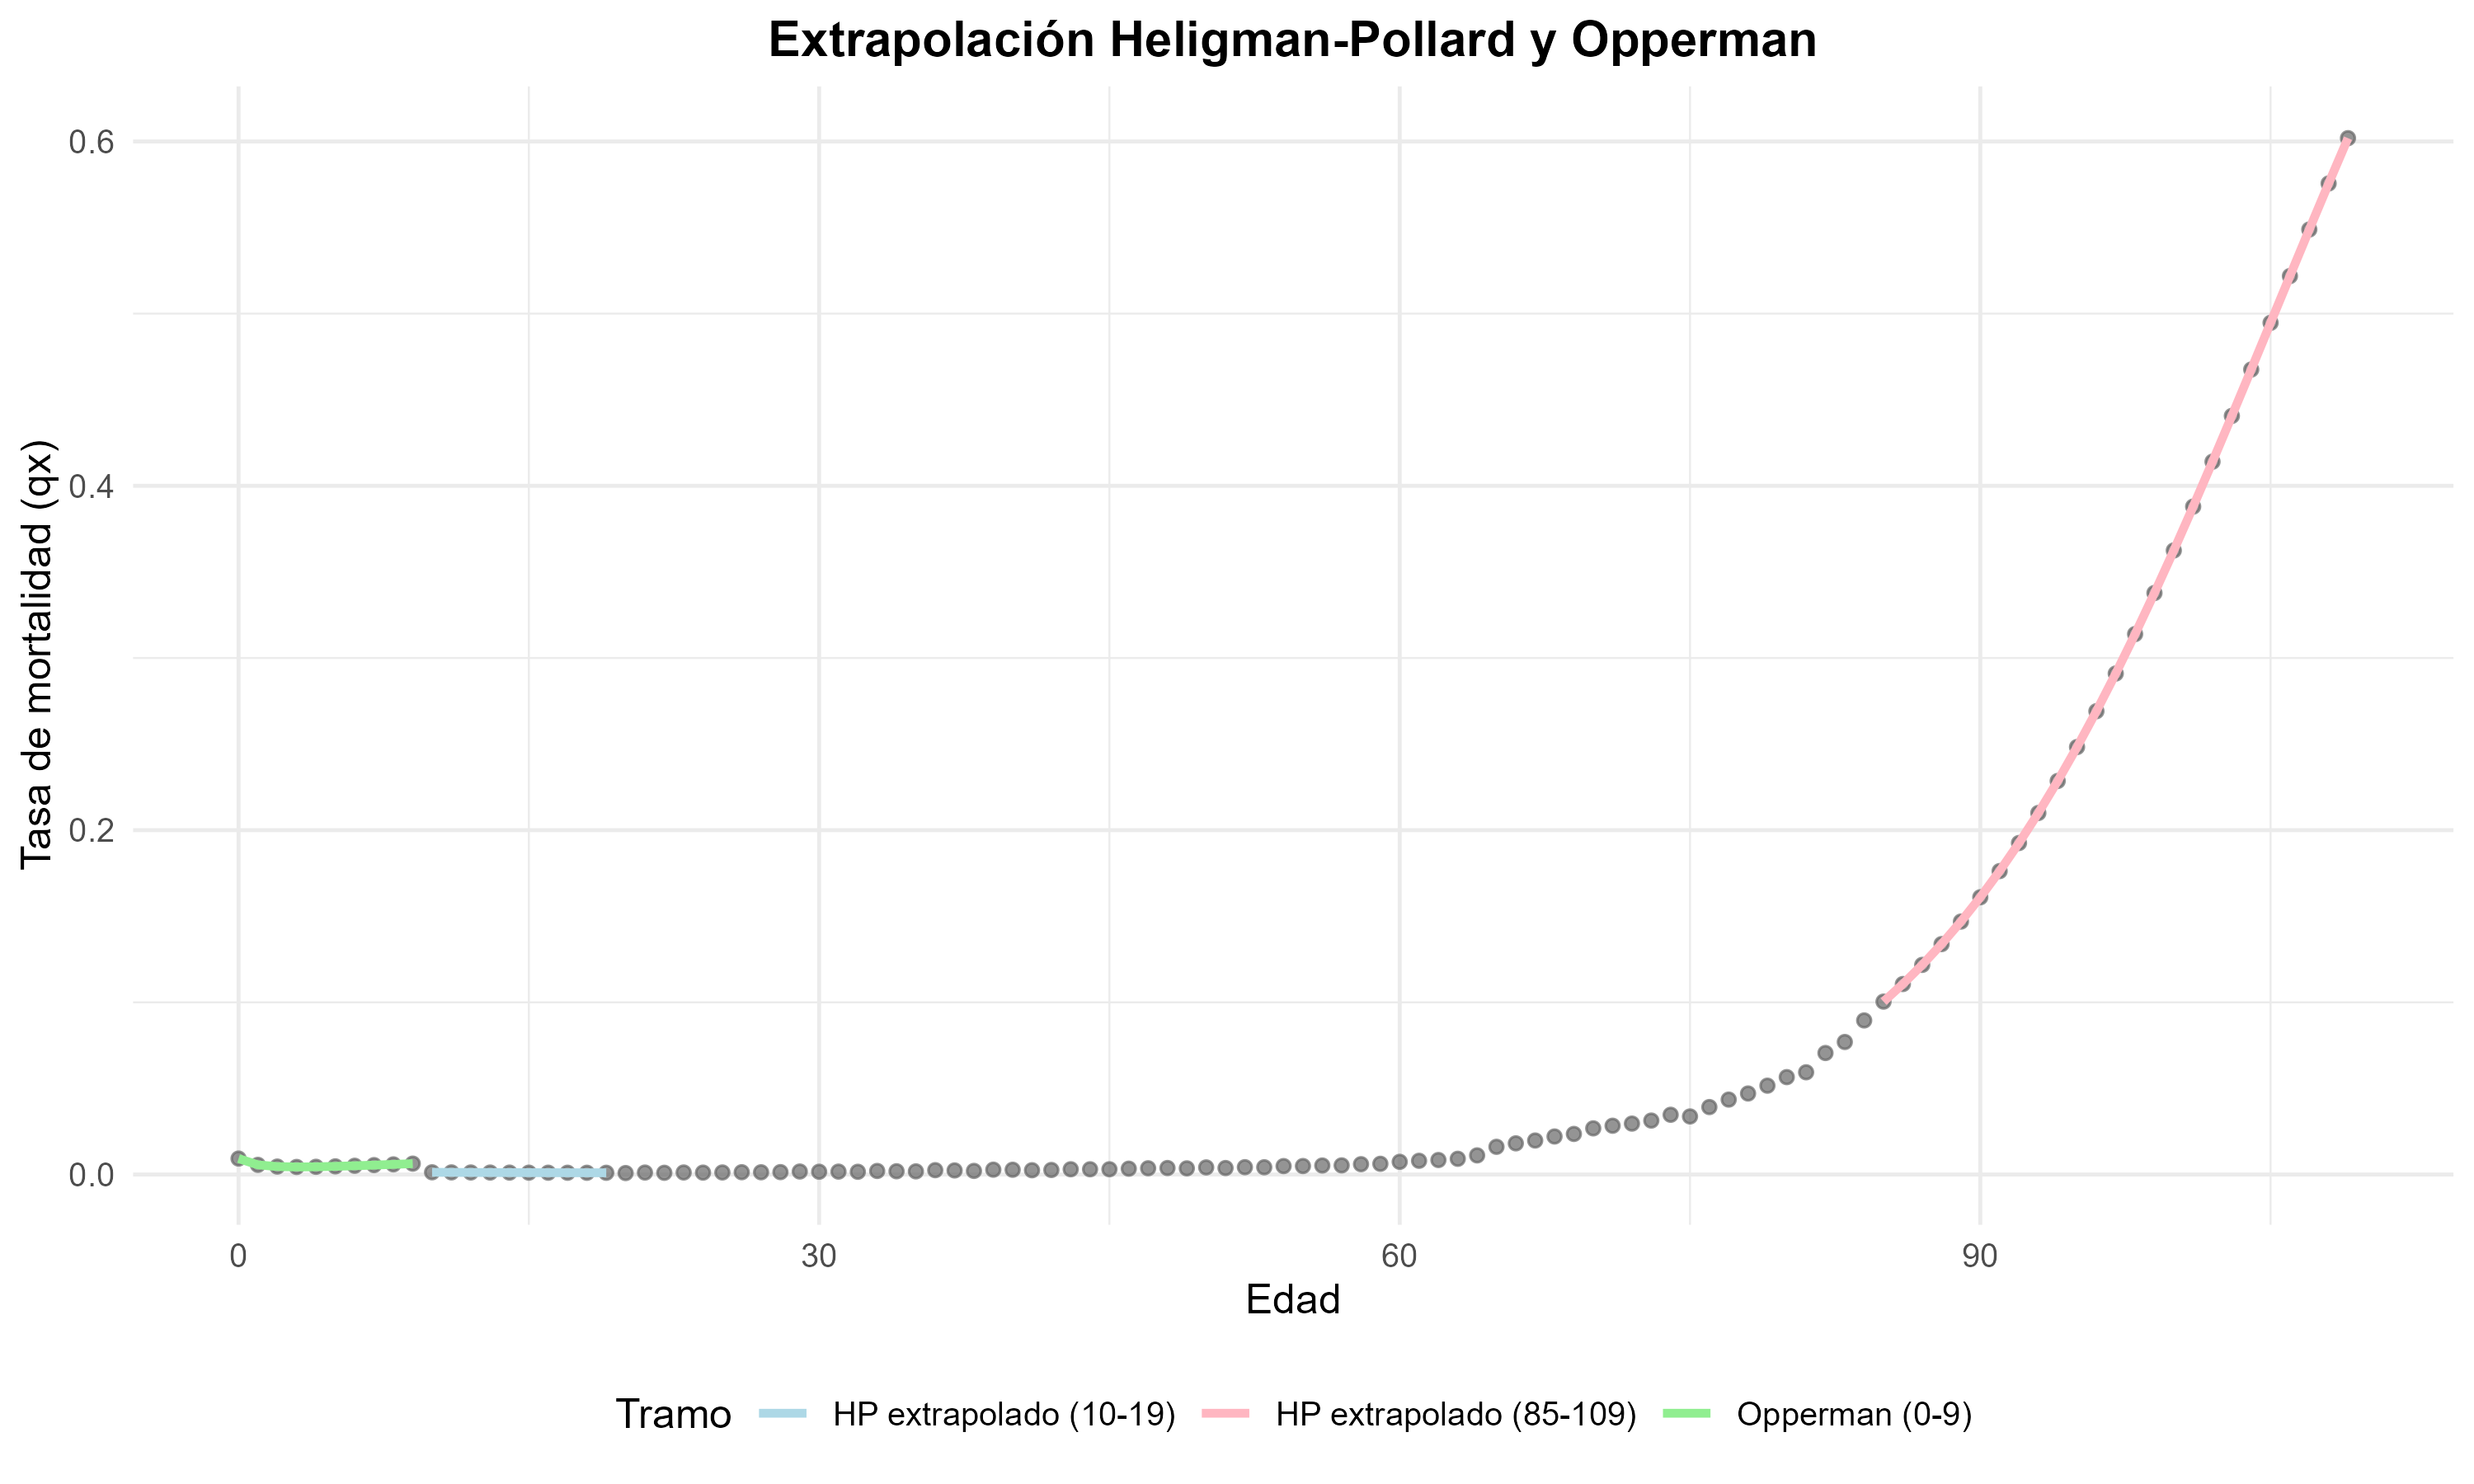
\includegraphics[width=0.85\textwidth]{Imagenes/05_extrapolacion_completa.png}
\caption{Tabla de mortalidad completa con extrapolaciones de Oppermann (0-19) y Heligman-Pollard (85-109)}
\label{fig:extrapolacion_completa}
\end{figure}

% ----------------------------------------------------------------------------
\subsection{Completar Tablas}

\subsubsection{Tabla Obtenida - Completa}

Se construyó la tabla completa de mortalidad con raíz $l_{10} = 10.000.000$, incluyendo todas las funciones biométricas:

\begin{itemize}
    \item $\qx{x}$: Probabilidad de muerte entre edad $x$ y $x+1$
    \item $\px{x}$: Probabilidad de sobrevivencia entre edad $x$ y $x+1$
    \item $\lx{x}$: Número de sobrevivientes a edad $x$
    \item $\dx{x}$: Número de muertes entre edad $x$ y $x+1$
    \item $\Lx{x}$: Años-persona vividos entre edad $x$ y $x+1$
    \item $\Tx{x}$: Años-persona totales a partir de edad $x$
    \item $\ex{x}$: Esperanza de vida a edad $x$
\end{itemize}

\begin{notabox}
\textbf{Nota:} La tabla completa se encuentra en el archivo: \texttt{tablas/tabla\_mortalidad\_obtenida.csv}

Por razones de espacio, se presenta aquí una versión resumida. La tabla completa está disponible en el repositorio del proyecto.
\end{notabox}

\begin{table}[H]
\centering
\caption{Tabla de mortalidad obtenida (extracto) - Edades seleccionadas}
\label{tab:tabla_obtenida_extracto}
\small
\begin{tabular}{ccccccc}
\toprule
\tableheadercolor
\textbf{Edad} & $\mathbf{q_x}$ & $\mathbf{p_x}$ & $\mathbf{l_x}$ & $\mathbf{d_x}$ & $\mathbf{L_x}$ & $\mathbf{e_x}$ \\
\midrule
0 & 0.002157 & 0.997843 & 10,000,000 & 21,570 & 9,989,215 & 18.88 \\
25 & 0.000734 & 0.999266 & 9,889,562 & 7,260 & 9,885,932 & 18.40 \\
45 & 0.003084 & 0.996916 & 9,692,820 & 29,892 & 9,677,874 & 16.06 \\
65 & 0.015831 & 0.984169 & 8,774,333 & 138,917 & 8,704,875 & 11.06 \\
85 & 0.111845 & 0.888155 & 5,012,948 & 560,600 & 4,732,648 & 4.86 \\
100 & 0.327823 & 0.672177 & 844,157 & 276,704 & 705,805 & 1.87 \\
109 & 1.000000 & 0.000000 & 65,332 & 65,332 & 32,666 & 0.50 \\
\bottomrule
\end{tabular}
\end{table}

\subsubsection{Gráfico Comparativo de Tasas de Mortalidad}

La Figura~\ref{fig:tasas_crudas} muestra las tasas de mortalidad observadas (crudas) antes del proceso de graduación:

\begin{figure}[H]
\centering
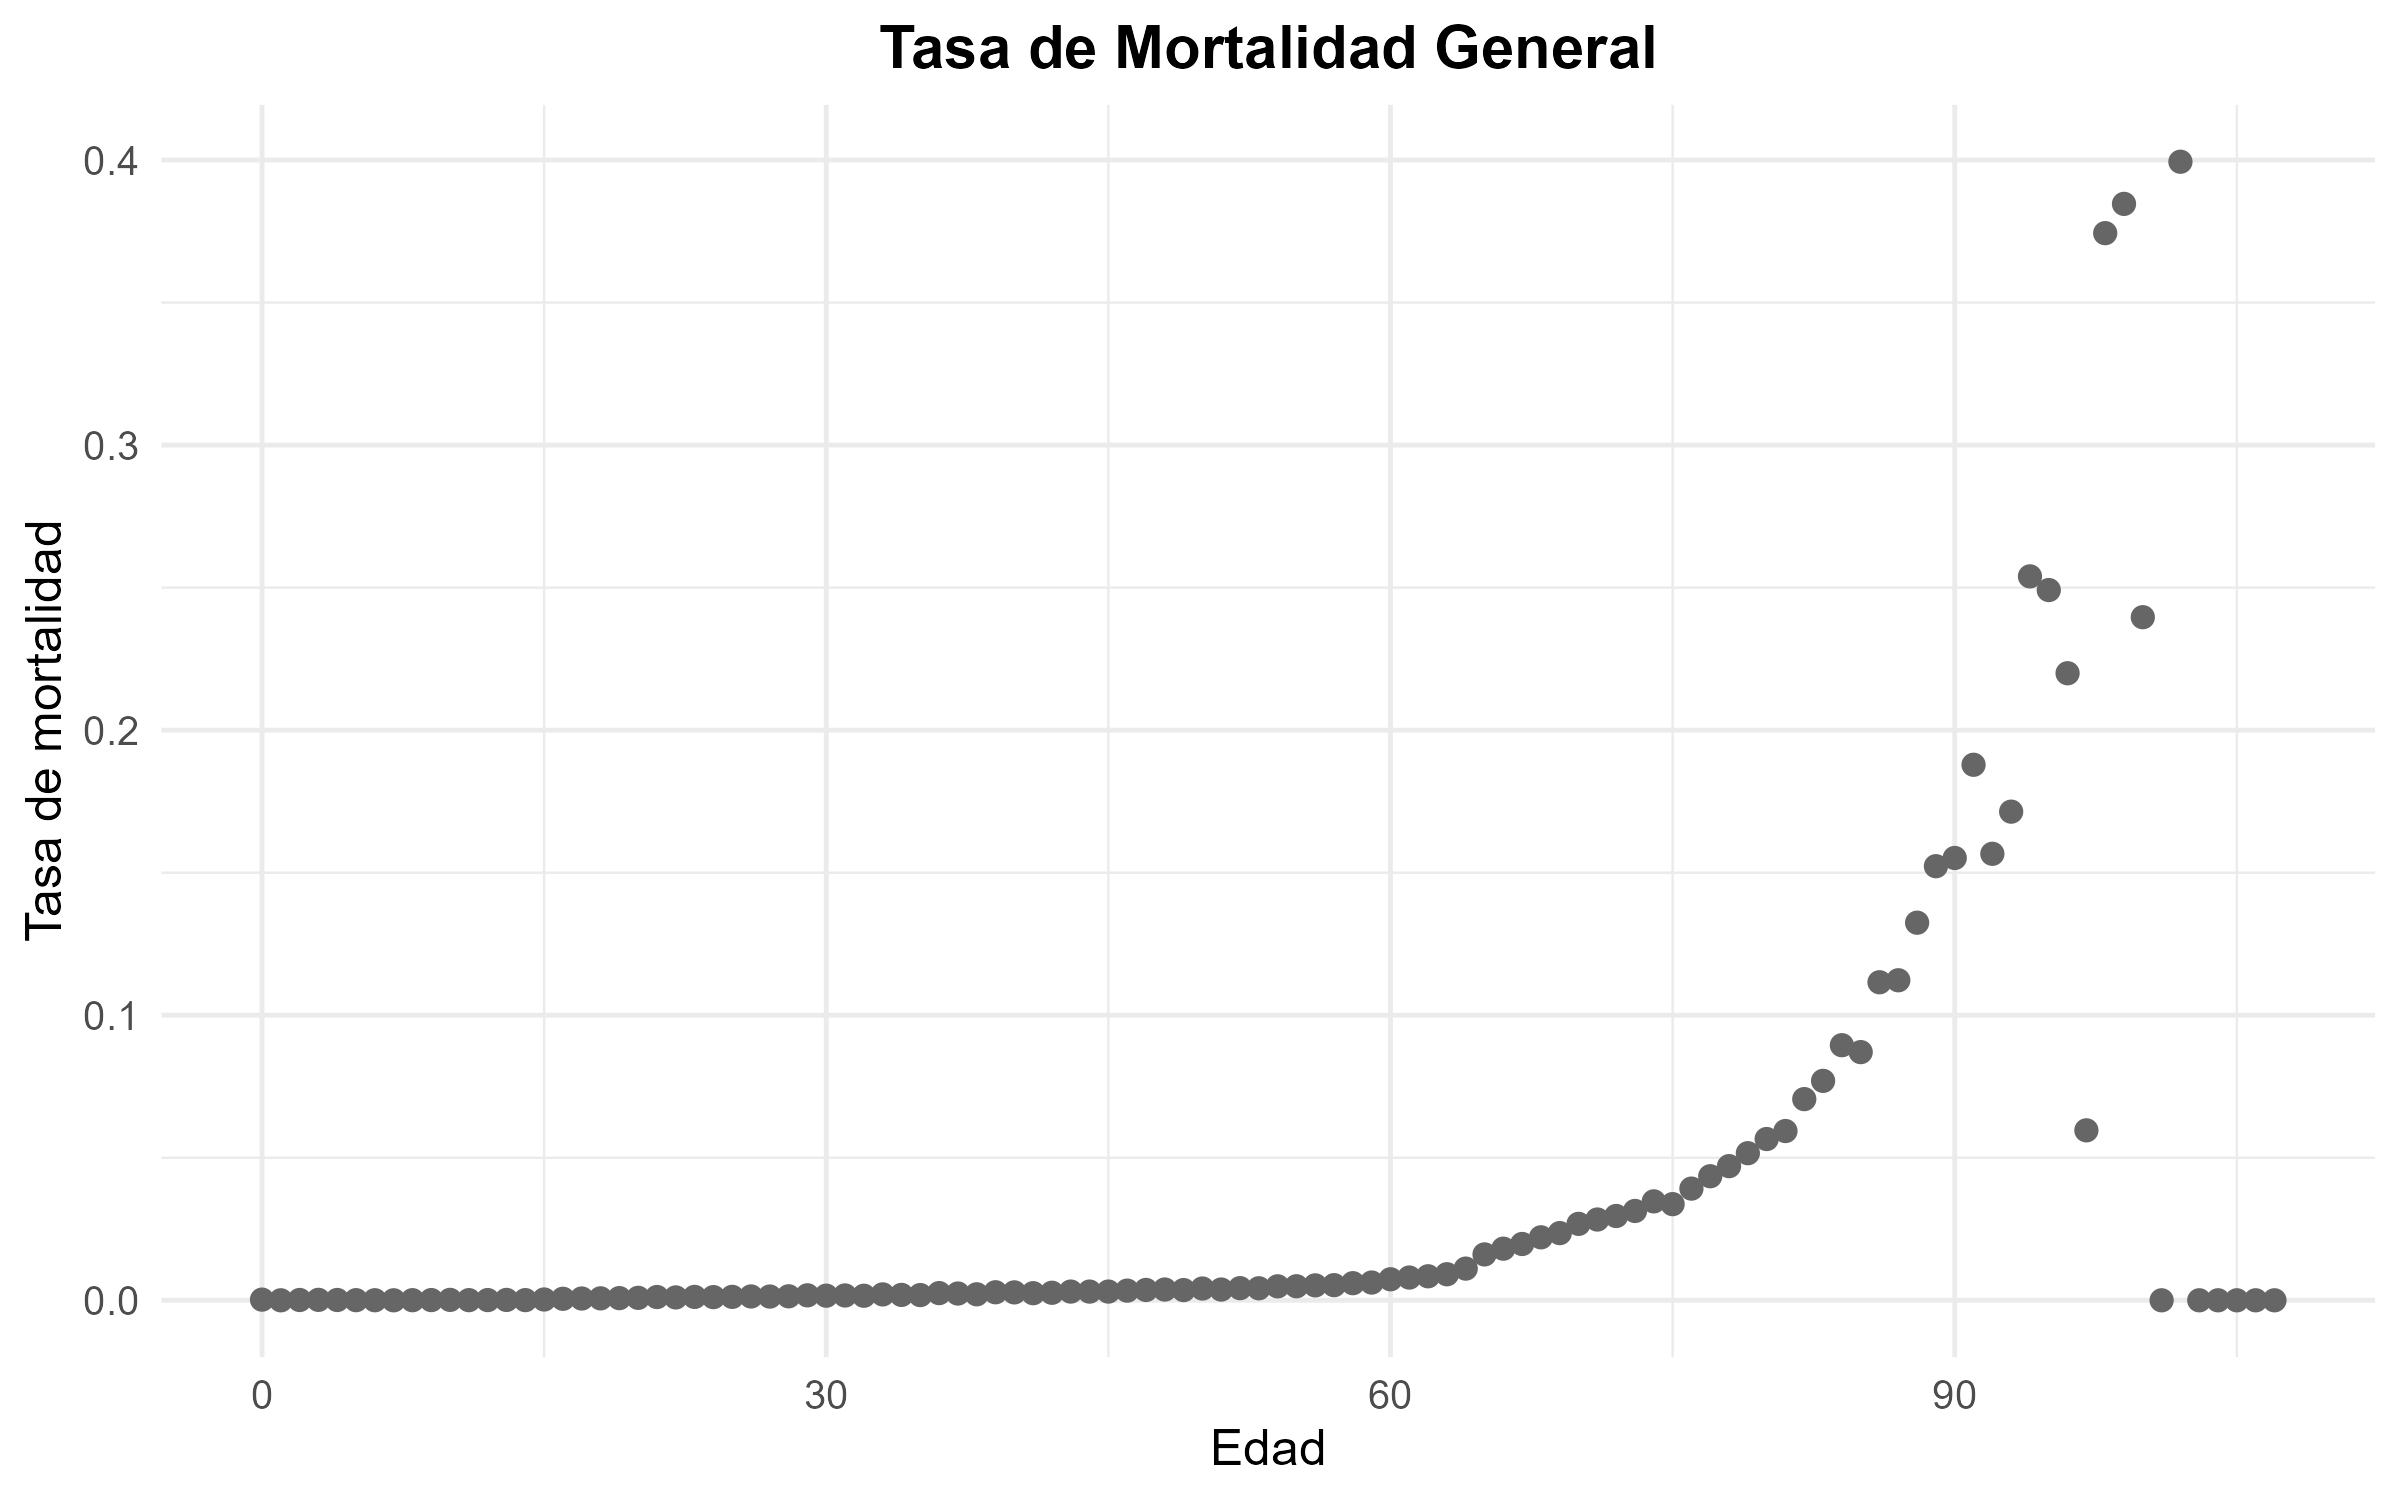
\includegraphics[width=0.85\textwidth]{Imagenes/01_tasa_mortalidad_general.png}
\caption{Tasas de mortalidad crudas observadas en la población de estudio}
\label{fig:tasas_crudas}
\end{figure}

La Figura~\ref{fig:graduacion_wh} presenta las tasas graduadas utilizando el método Whittaker-Henderson:

\begin{figure}[H]
\centering
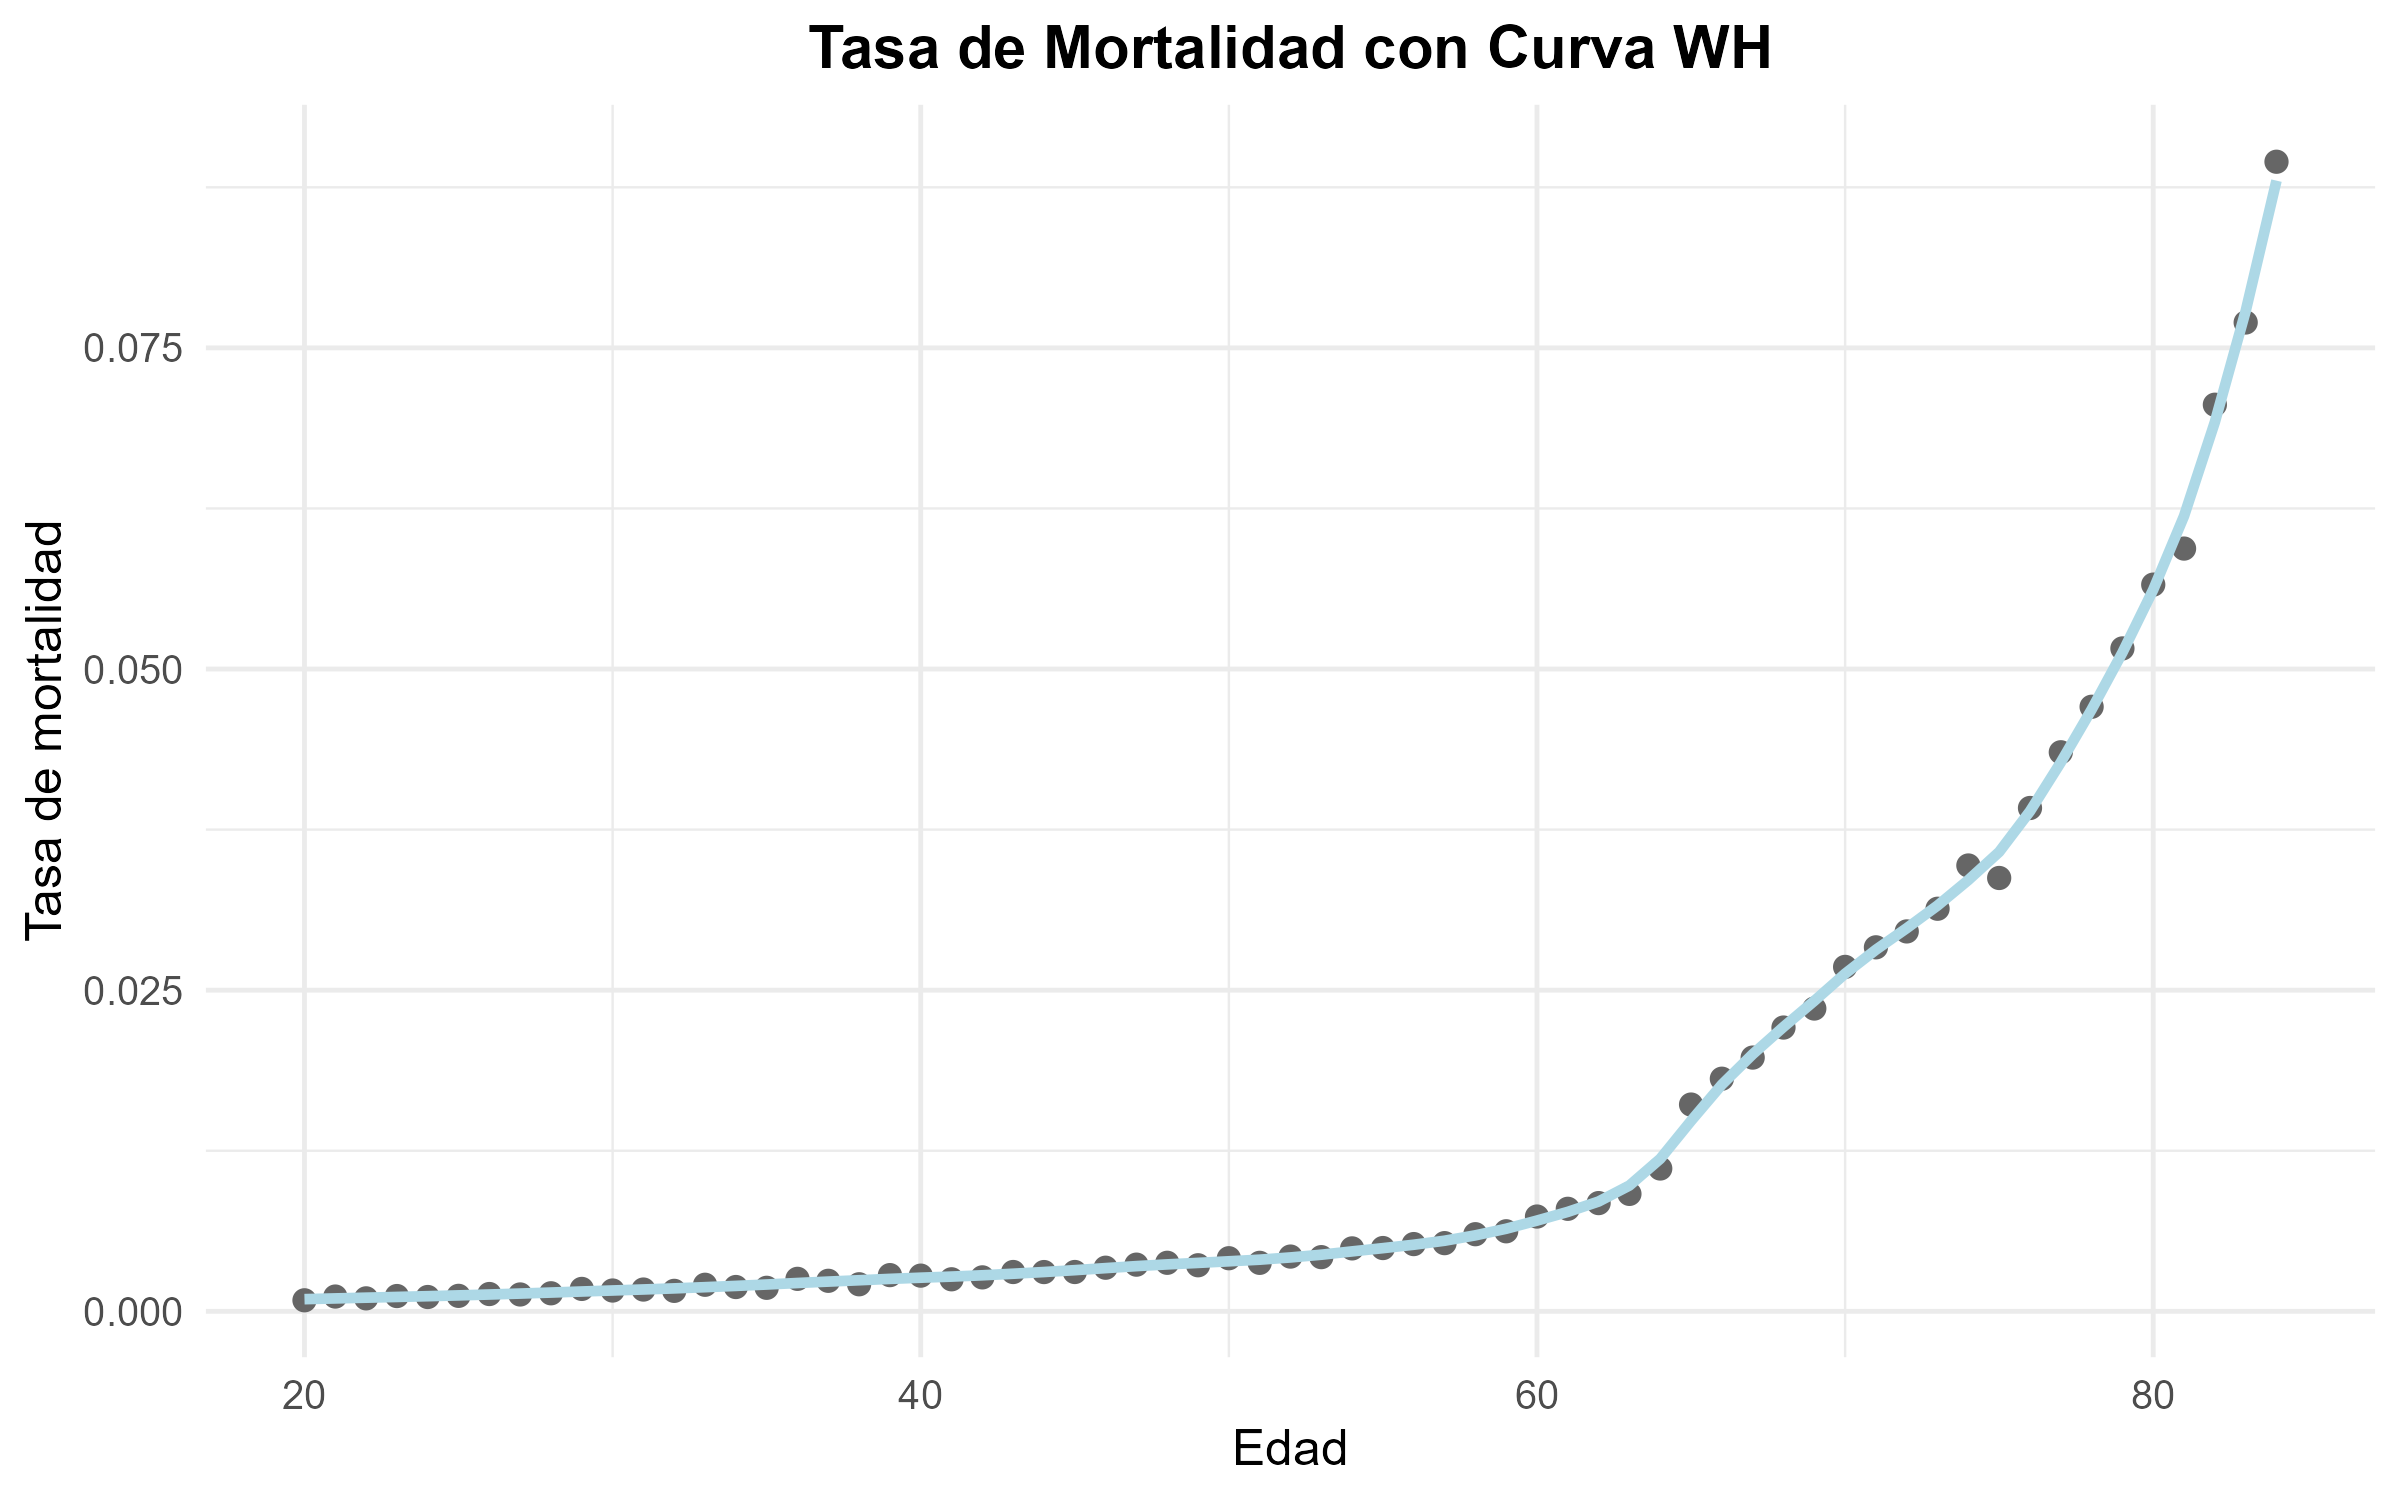
\includegraphics[width=0.85\textwidth]{Imagenes/02_tasa_mortalidad_WH.png}
\caption{Tasas de mortalidad graduadas con Whittaker-Henderson}
\label{fig:graduacion_wh}
\end{figure}

La Figura~\ref{fig:graduacion_completa} muestra la comparación final entre tasas crudas y graduadas:

\begin{figure}[H]
\centering
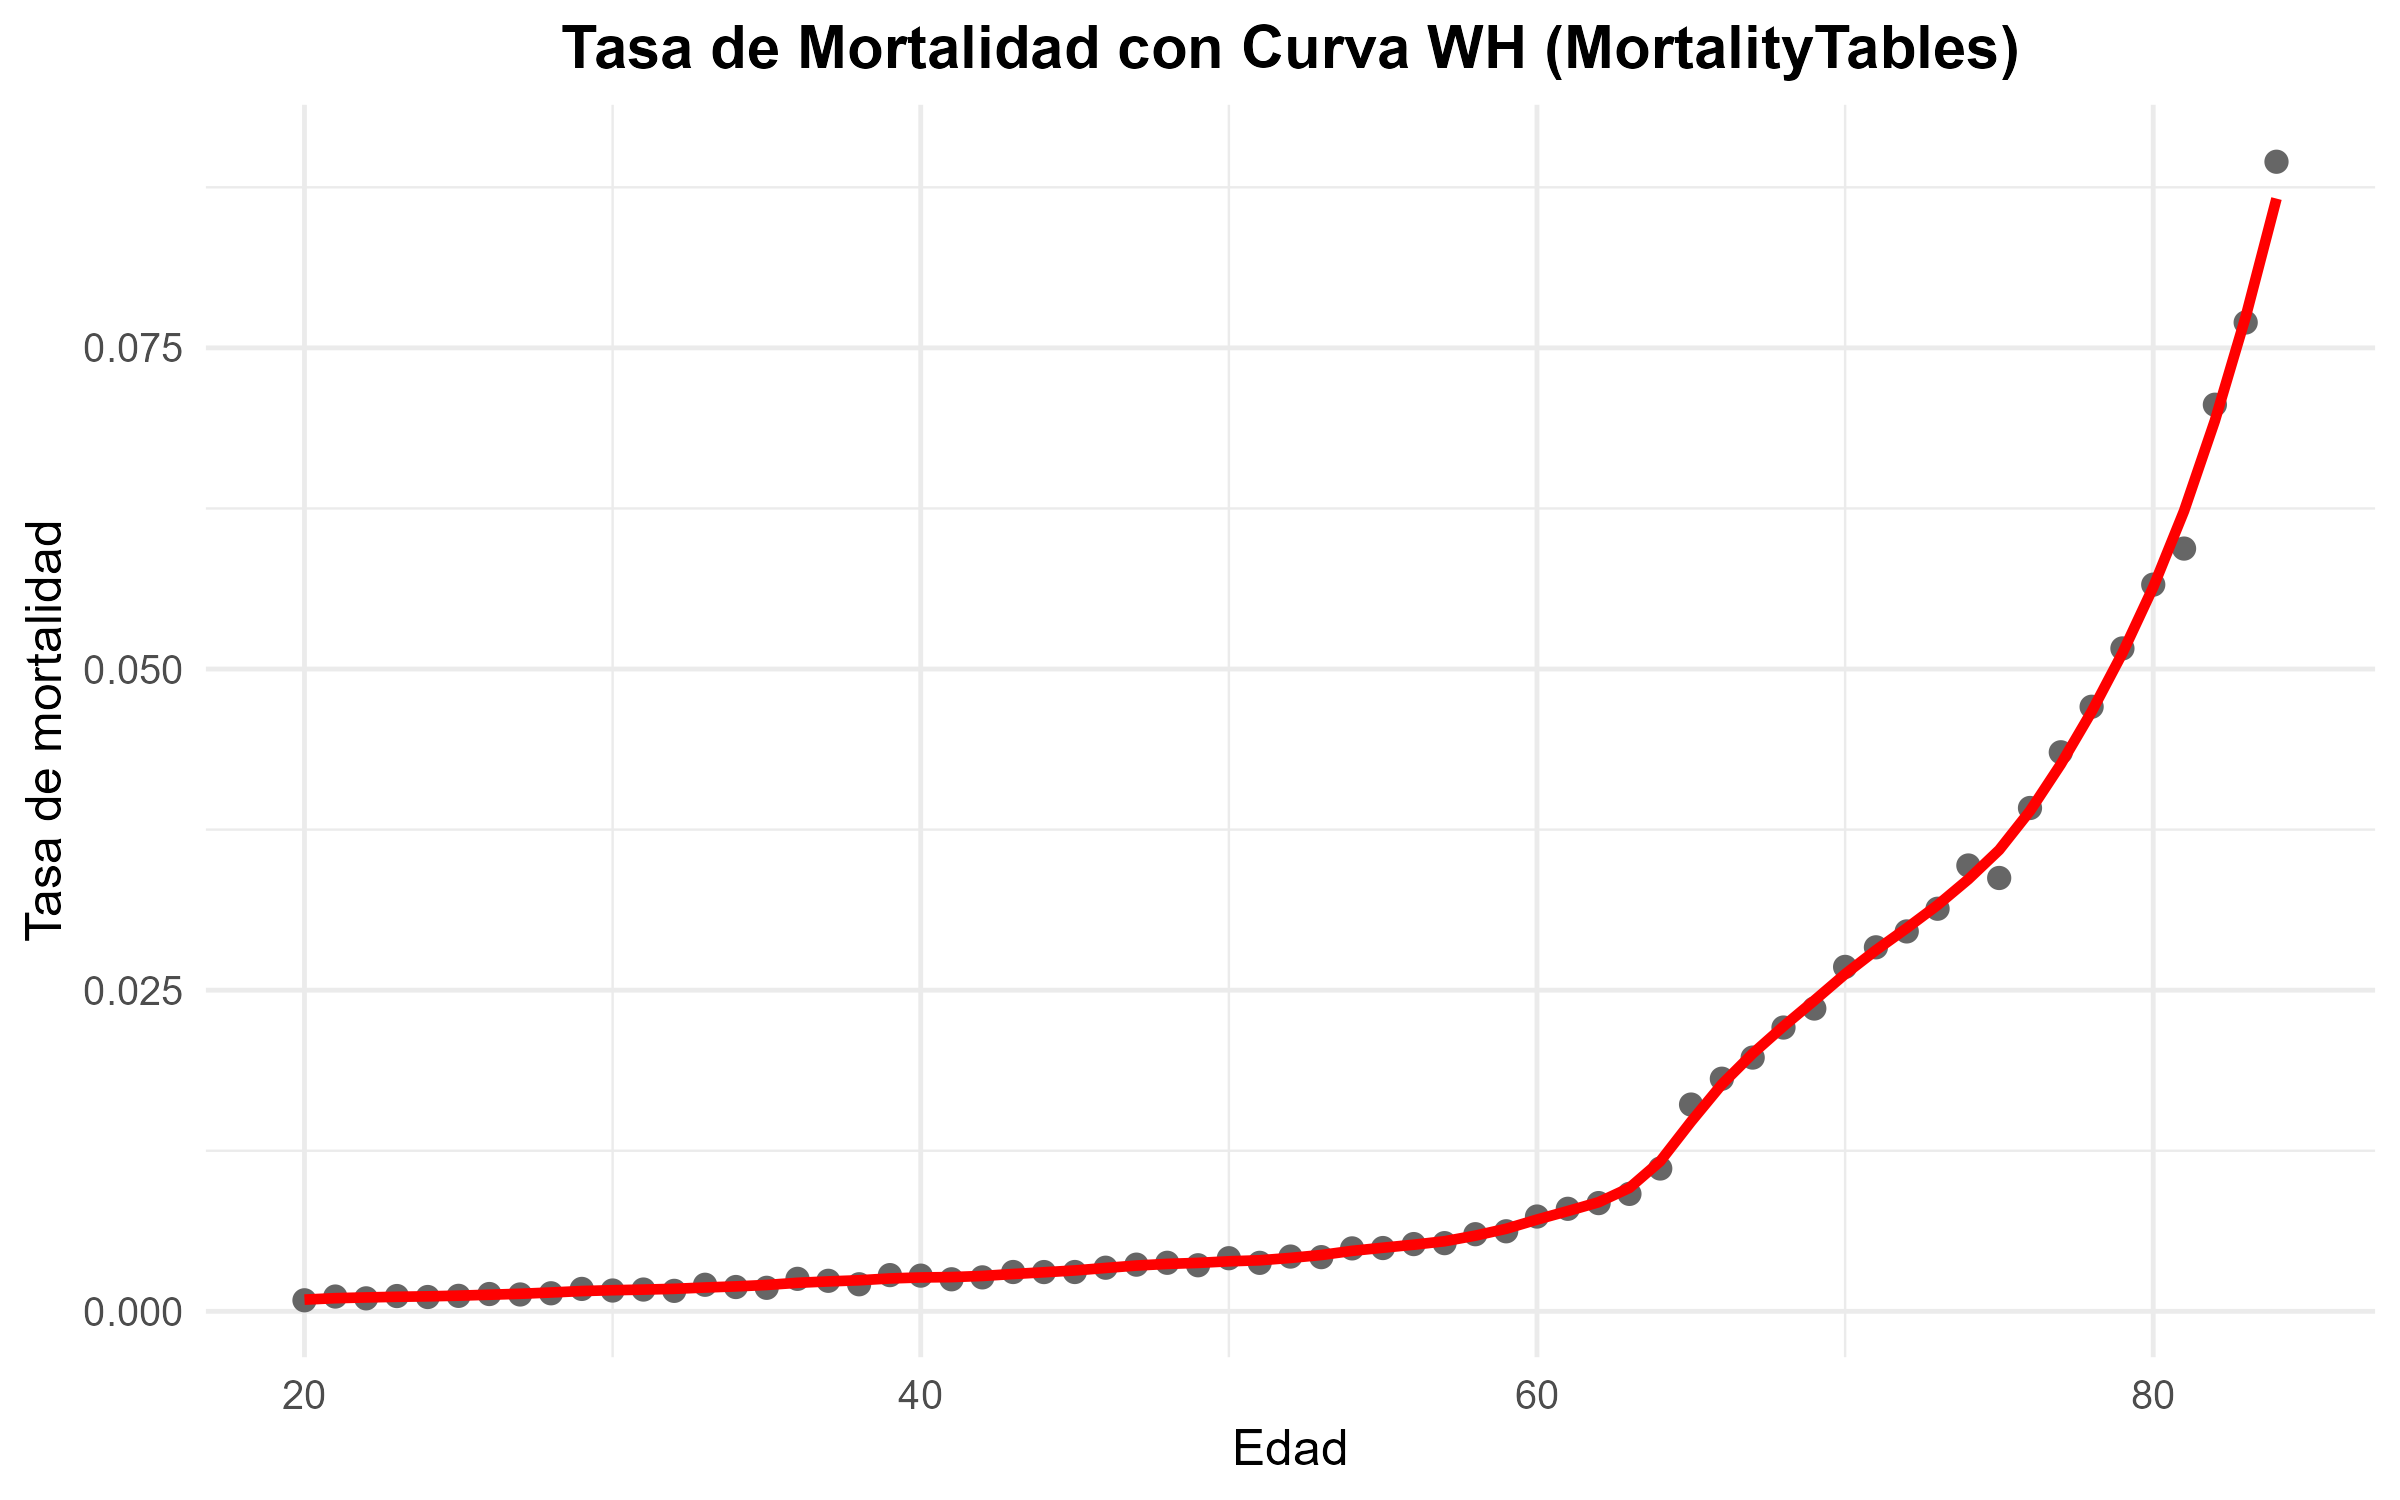
\includegraphics[width=0.85\textwidth]{Imagenes/03_tasa_mortalidad_WH_MortalityTables.png}
\caption{Comparación tasas crudas vs. graduadas (Método Whittaker-Henderson)}
\label{fig:graduacion_completa}
\end{figure}

Se observa que el método de graduación logra suavizar efectivamente las irregularidades de las tasas crudas, manteniendo la tendencia general de crecimiento exponencial con la edad.

\subsubsection{Análisis de Esperanza de Vida}

\begin{hallazgobox}
\textbf{Esperanzas de vida clave:}
\begin{itemize}
    \item $e_{0}$ = 18.88 años
    \item $e_{25}$ = 18.40 años
    \item $e_{45}$ = 16.06 años
    \item $e_{65}$ = 11.06 años
    \item $e_{85}$ = 4.86 años
    \item $e_{100}$ = 1.87 años
\end{itemize}
\end{hallazgobox}

\textbf{Comparación con tabla de referencia MI2014:}

[COMPLETAR: Comentar las diferencias observadas en las esperanzas de vida respecto a la tabla de referencia y posibles explicaciones.]
